% Sections III-V of "Evidence-Grounded Generative AI Model for Engineering Research Document Citation".
% Compiles on its own (pdflatex, twice). To merge into the full paper, copy everything between
% "BEGIN BODY" and "END BODY" into the main .tex before the reference list, and copy the two
% counter lines away. Numbers in Section IV come from generated/results.tex, which
% eval/make_report.py rewrites after an evaluation run.
\documentclass[10pt,twocolumn,letterpaper]{article}
\usepackage[T1]{fontenc}
\usepackage{mathptmx}
\usepackage[left=45pt,right=43pt,top=54pt,bottom=56pt,columnsep=12pt]{geometry}
\usepackage{titlesec,caption,booktabs,tabularx,array,graphicx,amsmath,microtype}
\usepackage{algorithm,algpseudocode}
\usepackage{tikz}
\usetikzlibrary{arrows.meta,positioning,fit,backgrounds}
\usepackage[hidelinks]{hyperref}

\titleformat{\section}{\centering\normalsize\scshape}{\Roman{section}.}{0.5em}{}
\titlespacing*{\section}{0pt}{10pt plus 2pt}{5pt}
\titleformat{\subsection}{\normalsize\itshape}{\Alph{subsection}.}{0.5em}{}
\titlespacing*{\subsection}{0pt}{8pt plus 2pt}{3pt}
\renewcommand{\thetable}{\Roman{table}}
\captionsetup[table]{font={footnotesize,sc},labelfont=up,labelsep=newline,justification=centering,name=TABLE,skip=4pt}
\captionsetup[figure]{font=footnotesize,labelsep=period,name=Fig.,justification=justified,singlelinecheck=false,skip=5pt}
\captionsetup[algorithm]{font=footnotesize}
\setlength{\parindent}{10pt}
\setlength{\textfloatsep}{10pt plus 2pt}
\setlength{\dbltextfloatsep}{10pt plus 2pt}
\setlength{\tabcolsep}{4pt}
\algrenewcommand\algorithmicrequire{\textbf{Input:}}
\algrenewcommand\algorithmicensure{\textbf{Output:}}
\algrenewcommand\alglinenumber[1]{\scriptsize #1:}
\newcommand{\todo}[1]{\par\smallskip\noindent\fbox{\parbox{0.955\columnwidth}{\footnotesize\raggedright\textbf{To fill after the run.} #1}}\par\smallskip}
% Generated by eval/make_report.py - do not edit by hand.
\newcommand{\ResLLM}{--}
\newcommand{\ResEmbedder}{--}
\newcommand{\ResJudge}{--}
\newcommand{\ResDate}{--}
\newcommand{\ResNPapers}{12}
\newcommand{\ResNChunks}{--}
\newcommand{\ResNAsk}{30}
\newcommand{\ResNCross}{6}
\newcommand{\ResNUnans}{4}
\newcommand{\ResNPaperTasks}{6}
\newcommand{\ResCRbase}{--}
\newcommand{\ResCPbase}{--}
\newcommand{\ResFAbase}{--}
\newcommand{\ResCRdraft}{--}
\newcommand{\ResCPdraft}{--}
\newcommand{\ResFAdraft}{--}
\newcommand{\ResCRver}{--}
\newcommand{\ResCPver}{--}
\newcommand{\ResFAver}{--}
\newcommand{\ResRefTotal}{--}
\newcommand{\ResRefChecked}{--}
\newcommand{\ResRefFab}{--}
\newcommand{\ResRefFabPct}{--}
\newcommand{\ResRefInCorpus}{--}
\newcommand{\ResRefOutside}{--}
\newcommand{\ResRefUnchecked}{--}
\newcommand{\ResRefErr}{--}
\newcommand{\ResRefErrPct}{--}
\newcommand{\ResDraftN}{--}
\newcommand{\ResRemovedN}{--}
\newcommand{\ResRemovedPct}{--}
\newcommand{\ResAbstainSys}{--}
\newcommand{\ResAbstainBase}{--}
\newcommand{\ResFalseAbstain}{--}
\newcommand{\ResSecBase}{--}
\newcommand{\ResSecDraft}{--}
\newcommand{\ResSecVer}{--}
\newcommand{\ResCallsVer}{--}
\newcommand{\ResUncitedBase}{--}
\newcommand{\ResNote}{}
\newcommand{\ResTableMain}{%
\begin{tabular}{@{}lcccccc@{}}
\toprule
System & Cit.\ rec. & Cit.\ prec. & Faithf. & Stmts & Calls & Time (s) \\
\midrule
Plain LLM (no documents) & -- & -- & -- & -- & -- & -- \\
Grounded, no verification & -- & -- & -- & -- & -- & -- \\
Grounded + verification & -- & -- & -- & -- & -- & -- \\
\bottomrule
\end{tabular}}
\newcommand{\ResTableRefs}{%
\begin{tabular}{@{}lcc@{}}
\toprule
Reference status & Count & Share (\%) \\
\midrule
Not found in any registry (fabricated) & -- & -- \\
Real, in the corpus & -- & -- \\
Real, outside the corpus & -- & -- \\
\midrule
Real but wrong year or first author & -- & -- \\
Could not be checked (no registry reachable) & -- & n/a \\
\bottomrule
\end{tabular}}
\newcommand{\ResTableRetrieval}{%
\begin{tabular}{@{}lccc@{}}
\toprule
Retriever & Hit@$k$ (\%) & Gold coverage (\%) & MRR \\
\midrule
Dense only & -- & -- & -- \\
BM25 only & -- & -- & -- \\
Hybrid (RRF) & -- & -- & -- \\
\bottomrule
\end{tabular}}
\newcommand{\ResTableModes}{%
\begin{tabular}{@{}lccccc@{}}
\toprule
Mode & Cit.\ rec. & Cit.\ prec. & Faithf. & Plain LLM faithf. & Interp. \\
\midrule
Ask Research & -- & -- & -- & -- & -- \\
Explain Paper & -- & -- & -- & -- & -- \\
Summarize Paper & -- & -- & -- & -- & -- \\
\bottomrule
\end{tabular}}
\newcommand{\ResFigMain}{\fbox{\parbox[c][3.2cm][c]{0.92\columnwidth}{\centering\footnotesize Bar chart of Table~IV.\\Written to \texttt{generated/fig\_main.pdf} by \texttt{eval/make\_report.py} after the evaluation run.}}}


\begin{document}
\title{\vspace{-8pt}\LARGE Evidence-Grounded Generative AI Model for\\Engineering Research Document Citation\\[4pt]
\normalsize Part 2: Methodology, Results and Discussion, and Future Work}
\author{\normalsize Kartikey Mani Tripathi, Bayya Venkata Anvesh, Anish Dattatraya Tabib, and Dr.\ Evangeline D\\
\normalsize\itshape Dept.\ of Information Science and Engineering, M S Ramaiah Institute of Technology, Bengaluru, India}
\date{}
\maketitle
\setcounter{section}{2}  % continues after II. Literature Survey
\setcounter{table}{1}    % continues after Table I

% ============================== BEGIN BODY ==============================
\section{Methodology}
The system is a fixed pipeline with no trained component (Fig.~\ref{fig:arch}). A paper is ingested once: its text is extracted, its bibliographic fields are stored, and its body is cut into chunks that go into two indexes. Each request then runs four steps in order: hybrid retrieval, passage-first generation, claim verification, and citation rendering. Two models are used and both stay frozen: a sentence-embedding model for dense retrieval and one large language model (LLM) that is called once to generate and again to verify.

\begin{figure*}[t]
\centering
\resizebox{\textwidth}{!}{%
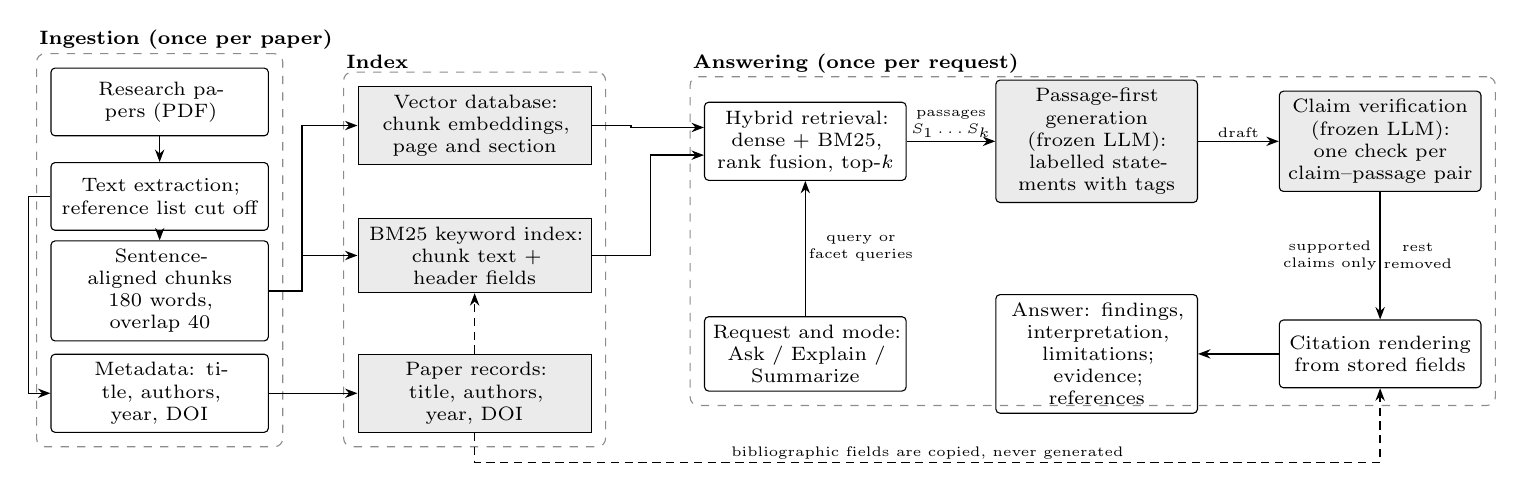
\begin{tikzpicture}[
  font=\scriptsize,
  box/.style={draw, rounded corners=1.5pt, align=center, inner sep=3pt, minimum height=0.86cm, text width=#1},
  box/.default=2.55cm,
  store/.style={draw, align=center, inner sep=3pt, minimum height=0.86cm, text width=2.75cm, fill=black!8},
  llm/.style={box=2.35cm, fill=black!8},
  flow/.style={-{Stealth[length=4.5pt]}, line width=0.5pt},
  note/.style={font=\tiny, align=center, inner sep=1pt},
  lane/.style={draw=black!45, dashed, rounded corners=3pt, inner sep=5pt},
  lanetitle/.style={font=\scriptsize\bfseries, anchor=south west, inner sep=1pt}]
% ---- ingestion
\node[box] (pdf)   at (1.55,4.75) {Research papers (PDF)};
\node[box] (parse) at (1.55,3.55) {Text extraction;\\reference list cut off};
\node[box] (chunk) at (1.55,2.35) {Sentence-aligned chunks\\180 words, overlap 40};
\node[box] (meta)  at (1.55,1.05) {Metadata: title, authors,\\year, DOI};
\draw[flow] (pdf) -- (parse);
\draw[flow] (parse) -- (chunk);
\draw[flow] (parse.west) -- ++(-0.28,0) |- (meta.west);
% ---- index
\node[store] (vec)  at (5.55,4.45) {Vector database:\\chunk embeddings,\\page and section};
\node[store] (bm)   at (5.55,2.80) {BM25 keyword index:\\chunk text + header fields};
\node[store] (rec)  at (5.55,1.05) {Paper records:\\title, authors, year, DOI};
\draw[flow] (chunk.east) -- ++(0.42,0) |- (vec.west);
\draw[flow] (chunk.east) -- ++(0.42,0) |- (bm.west);
\draw[flow] (meta) -- (rec);
\draw[flow, densely dashed] (rec) -- (bm);
% ---- answering
\node[box=2.35cm] (ret)  at (9.75,4.25)  {Hybrid retrieval:\\dense + BM25,\\rank fusion, top-$k$};
\node[llm]        (gen)  at (13.45,4.25) {Passage-first generation\\(frozen LLM): labelled statements with tags};
\node[llm]        (ver)  at (17.05,4.25) {Claim verification\\(frozen LLM): one check per claim--passage pair};
\node[box=2.35cm] (req)  at (9.75,1.55)  {Request and mode:\\Ask / Explain /\\Summarize};
\node[box=2.35cm] (ans)  at (13.45,1.55) {Answer: findings,\\interpretation, limitations;\\evidence; references};
\node[box=2.35cm] (rend) at (17.05,1.55) {Citation rendering\\from stored fields};
\draw[flow] (req) -- node[note, right] {query or\\facet queries} (ret);
\draw[flow] (vec.east) -- ++(0.5,0) |- ([yshift=5pt]ret.west);
\draw[flow] (bm.east) -- ++(0.75,0) |- ([yshift=-5pt]ret.west);
\draw[flow] (ret) -- node[note, above] {passages\\$S_1 \ldots S_k$} (gen);
\draw[flow] (gen) -- node[note, above] {draft} (ver);
\draw[flow] (ver) -- node[note, left] {supported\\claims only} node[note, right] {rest\\removed} (rend);
\draw[flow] (rend) -- (ans);
\draw[flow, densely dashed] (rec.south) -- ++(0,-0.38) -| node[note, pos=0.25, above] {bibliographic fields are copied, never generated} (rend.south);
% ---- lanes
\begin{scope}[on background layer]
\node[lane, fit=(pdf)(meta)(parse)] (l1) {};
\node[lane, fit=(vec)(rec)] (l2) {};
\node[lane, fit=(ret)(ver)(req)(rend)] (l3) {};
\end{scope}
\node[lanetitle] at (l1.north west) {Ingestion (once per paper)};
\node[lanetitle] at (l2.north west) {Index};
\node[lanetitle] at (l3.north west) {Answering (once per request)};
\end{tikzpicture}}
\caption{System architecture. Solid arrows carry text; dashed arrows carry stored bibliographic fields. Shaded boxes on the right are the two calls to the frozen LLM. Nothing in the pipeline is trained.}
\label{fig:arch}
\end{figure*}

\subsection{Ingestion and Metadata}
Text is read page by page from the PDF. Line-end hyphenation is repaired, bare page numbers are dropped, and section headings are detected from their numbering and from a list of common heading names, so every word keeps the page and the section it came from. Extraction stops at the reference list. This matters for citation quality: a bibliography entry mentions many topics in a few words and would otherwise be retrieved as if it were evidence.

Bibliographic fields are collected once, at this stage. The title is taken from the PDF metadata when it is usable and otherwise from the largest type on the first page; authors come from the metadata or the lines under the title; the DOI and arXiv identifier are matched by pattern on the first two pages. When an identifier is found the record can be replaced by the registry record (Crossref or arXiv), and a hand-checked side file overrides both. Each record keeps a field that says which of these sources it came from. The generator is never asked for a title, an author, a year, or a DOI, which removes the fabricated-reference failure measured in [2] and [3] by construction.

\subsection{Chunking and Indexing}
Whole sentences are packed into chunks of about 180 words. Consecutive chunks of a section share their trailing sentences, up to 40 words, and a chunk never crosses a section heading. Short chunks keep each prompt small and keep the evidence for a claim local, which follows the positional finding of [9].

Each chunk is stored twice. A sentence-embedding model maps it to a 384-dimensional unit vector that is stored in a vector database with its paper identifier, pages, and section. The same chunk, extended with its paper's title, authors, year, and DOI, is tokenised into a BM25 keyword index. The header fields are what let a typed surname or DOI reach the right paper even when the chunk never repeats them. Identifiers such as a DOI are indexed both whole and in parts. BM25 uses the form of inverse document frequency that stays positive, because in a session-sized corpus a paper's own identifiers occur in most of its chunks and the classic form would score them at zero.

\subsection{Hybrid Retrieval}
A request is turned into one or more queries (Table~\ref{tab:modes}). For each query the dense index and the keyword index each return their best $n=20$ chunks. The rankings are merged by reciprocal rank fusion,
\begin{equation}
s(c)=\sum_{r\in R}\frac{1}{\kappa+\operatorname{rank}_r(c)},\qquad \kappa=60,
\label{eq:rrf}
\end{equation}
where $R$ is the set of rankings that contain chunk $c$. Fusion works on ranks, so cosine similarities and BM25 scores never have to be put on one scale. The top $k$ chunks become the passages $S_1,\ldots,S_k$. This is the blended retrieval of [6] in a training-free form. Retrieval runs once per request; there is no second hop and no query rewriting.

\begin{table}[t]
\caption{The Three Modes}
\label{tab:modes}
\footnotesize
\begin{tabularx}{\columnwidth}{@{}>{\raggedright\arraybackslash}p{1.4cm}>{\raggedright\arraybackslash}p{0.95cm}Xc@{}}
\toprule
Mode & Scope & Queries and output & $k$\\
\midrule
Ask\newline Research & All papers & The question itself; at most four passages per paper. Three to seven statements. & 6\\
\addlinespace[2pt]
Explain\newline Paper & One paper & The user's focus, or five fixed facets. Headings: Problem, Method, Results, Key concepts, Limitations. & 8\\
\addlinespace[2pt]
Summarize\newline Paper & One paper & Six fixed facets. Headings: Objective, Method, Data and setup, Results, Limitations, Takeaway. & 10\\
\bottomrule
\end{tabularx}
\end{table}

\subsection{Passage-First Generation in Three Modes}
The three modes differ only in retrieval scope, queries, and the headings asked for (Table~\ref{tab:modes}); the grounding rule is shared. In the two single-paper modes the passages are put back in reading order before generation.

The prompt contains the passages and nothing else about the papers. Each passage is headed by its tag, paper, pages, and section. The LLM returns a list of statements, each one sentence with three fields: the text, a label, and the tags it rests on. The label is one of \emph{finding} (stated by a passage), \emph{limitation} (a limit the paper itself states), and \emph{interpretation} (the model's own explanation or comparison). The prompt forbids writing reference details, tells the model to split a sentence that mixes a passage's content with its own addition, and tells it to return an explicit ``insufficient'' flag instead of guessing. This is the select-then-write order of [12] without a separate span-selection model. A tag that was not in the prompt is discarded when the output is parsed, so the model cannot cite a source it was not shown.

\subsection{Claim Verification}
Verification is a separate call that sees only claims and passages, not the question or the draft as a whole. Every (statement, cited passage) pair is sent as one item, ten items per call. For each item the verifier returns one of four verdicts, \emph{full}, \emph{partial}, \emph{none}, or \emph{contradicted}, and for the first two the shortest span of the passage that supports the claim.

Three rules turn verdicts into the answer. (i) \emph{Quote anchoring}: a \emph{full} verdict counts only if the returned span is really in the passage, exactly or with at least 85 percent of its content words; otherwise it is lowered to \emph{partial}. This stops a verifier that agrees with the generator and invents its proof. (ii) A finding or limitation is kept if at least one cited passage supports it in full, and it keeps only those citations. If two or more passages support it in part, the claim is checked once more against them together, which covers statements that join two passages. Otherwise it is removed. (iii) An interpretation is kept when a cited passage gives it a full or partial basis and none contradicts it; it stays labelled as the system's reading.

Removed statements are not rewritten. As in [11] and [14] the check comes after generation, but the verifier here only deletes, so it cannot add a new unsupported sentence. Removed statements are shown to the user in a separate list with the reason. If a verification call fails, its items count as unsupported.

\subsection{Citation Rendering and Abstention}
Kept statements are numbered against their passages in order of first use. Each evidence entry shows the paper, pages, section, and the anchored span; the reference list is formatted in IEEE style from the stored record of each cited paper. If retrieval returns nothing, the generator flags the passages as insufficient, or no statement survives verification, the system says that the uploaded papers do not contain the evidence and gives no answer.

\begin{algorithm}[t]
\caption{Evidence-grounded answering}
\label{alg:main}
\footnotesize
\begin{algorithmic}[1]
\Require request $q$, mode $m$, paper filter $p$ (or none), indexes $I$
\Ensure statements $A$ with evidence and references, or \textsc{decline}
\State $Q \gets$ \textsc{Queries}$(q,m)$;\ \ $R\gets\emptyset$ \Comment{$q$ itself or fixed facets}
\ForAll{$q_i \in Q$}
  \State $R \gets R \cup \{\textsc{Dense}(I,q_i,n,p),\ \textsc{BM25}(I,q_i,n,p)\}$
\EndFor
\State $P \gets$ top-$k$ chunks by $s(c)$ in (\ref{eq:rrf}), tagged $S_1..S_k$
\If{$P=\emptyset$} \Return \textsc{decline} \EndIf
\State $D \gets \textsc{Generate}(m,P)$ \Comment{LLM call 1: text, label, tags}
\State drop from every $d\in D$ the tags that are not in $P$
\State $V \gets \textsc{Verify}(\{(d,t): d\in D,\ t\in d.\mathit{tags}\})$ \Comment{LLM call 2}
\ForAll{$(d,t)$ with $V_{d,t}=\textit{full}$ and span not found in $P_t$}
  \State $V_{d,t}\gets\textit{partial}$ \Comment{quote anchoring}
\EndFor
\State $A\gets\emptyset$
\ForAll{$d\in D$}
  \State $F\gets\{t: V_{d,t}=\textit{full}\}$;\ \ $H\gets\{t: V_{d,t}=\textit{partial}\}$
  \If{$d$ is a finding or limitation}
    \If{$F\neq\emptyset$} $A\gets A\cup\{d \text{ citing } F\}$
    \ElsIf{$|H|\ge 2$ \textbf{and} $\textsc{Verify}(d,\textstyle\bigcup_{t\in H}P_t)=\textit{full}$}
      \State $A\gets A\cup\{d \text{ citing } H\}$
    \EndIf \Comment{else $d$ is removed}
  \ElsIf{$F\cup H\neq\emptyset$ \textbf{and} no $V_{d,t}=\textit{contradicted}$}
    \State $A\gets A\cup\{d \text{ citing } F\cup H\}$ \Comment{interpretation}
  \EndIf
\EndFor
\If{$A=\emptyset$} \Return \textsc{decline} \EndIf
\State \Return $A$, cited passages, stored records of their papers
\end{algorithmic}
\end{algorithm}

\subsection{Algorithm and Cost}
Algorithm~\ref{alg:main} gives the full request path. A request costs one generation call and $\lceil N/10\rceil$ verification calls for $N$ claim--passage pairs, plus at most one call for the joint check. With the statement counts in Table~\ref{tab:modes} this is two to four LLM calls per request. Retrieval is two index lookups per query and needs no LLM.

\begin{table}[t]
\caption{Implementation Parameters}
\label{tab:params}
\footnotesize
\begin{tabularx}{\columnwidth}{@{}lX@{}}
\toprule
Component & Setting\\
\midrule
PDF parsing & PyMuPDF; reference list excluded\\
Chunking & 180 words, whole sentences, overlap up to 40 words\\
Dense retrieval & all-MiniLM-L6-v2, 384-d, cosine; ChromaDB\\
Keyword retrieval & BM25, $k_1=1.5$, $b=0.75$, positive IDF\\
Fusion & Reciprocal rank fusion, $\kappa=60$, $n=20$ per ranking\\
Generator and verifier & One frozen LLM, temperature 0, JSON output\\
Verification & 10 pairs per call; quote anchor at 0.85\\
Interface & Streamlit web app and command line\\
\bottomrule
\end{tabularx}
\end{table}

\subsection{Implementation}
The system is written in Python (Table~\ref{tab:params}). The LLM is reached through the OpenAI-compatible chat interface, so a hosted model and a local one are interchangeable without code changes; every parameter in Table~\ref{tab:params} is read from one configuration file. The web interface has one tab per mode. It shows each statement with its label and evidence numbers, opens the cited passage with the supporting span highlighted, and lists the removed statements. A test suite runs the whole pipeline offline with a scripted model to check the rules of Section~III-E.

\section{Results and Discussion}
\ResNote
\subsection{Experimental Setup}
\emph{Corpus.} The corpus has \ResNPapers{} research papers on retrieval-augmented generation, attribution, and their evaluation, taken from the works reviewed in Section~II and indexed as \ResNChunks{} chunks. Their metadata was taken from the arXiv record.

\emph{Requests.} There are \ResNAsk{} Ask Research questions, each with the paper or papers that contain its answer marked as gold; \ResNCross{} of them need two papers. A further \ResNUnans{} questions are on engineering topics that no paper in the corpus covers. Explain Paper and Summarize Paper are each run on \ResNPaperTasks{} papers.

\emph{Systems.} Three systems answer every request with the same frozen LLM (\ResLLM): (a) the plain LLM, which sees no documents and is asked for statements with numbered references; (b) the grounded system without verification; and (c) the full system. Systems (b) and (c) share one generation, so any difference between them is due to verification alone.

\subsection{Metrics}
All metrics are computed over statements and micro-averaged. Support is judged by a natural-language-inference cross-encoder (nli-deberta-v3-base, entailment probability at least 0.5) that is not used inside the system, as in [10].

\emph{Citation recall} is the share of findings and limitations that are entailed by the passages they cite. \emph{Citation precision} is the share of citations that support their statement, that is, the passage entails the statement alone or the statement loses its support without it [10]. \emph{Faithfulness} is the share of statements entailed by at least one of the five corpus passages retrieved for that statement; it follows the supported-claims ratio of [19] and the retrieve-then-check procedure of [20], and it is computed the same way for all three systems.

The plain LLM cites references, not passages, so its citations are scored at paper level. Each reference is first classified: in the corpus, real but outside it (found by title in Crossref, OpenAlex, or arXiv), or not found in any registry. A citation counts as supporting when its reference is in the corpus and a passage of that paper entails the statement. References that are real but outside the corpus cannot be checked against text and are left out of precision; references not found anywhere count as unsupported.

\subsection{Citation Quality and Faithfulness}
\begin{table}[t]
\caption{Main Comparison (percent, except the last three columns)}
\label{tab:main}
\footnotesize\setlength{\tabcolsep}{3pt}
\resizebox{\columnwidth}{!}{\ResTableMain}
\end{table}

Table~\ref{tab:main} and Fig.~\ref{fig:main} give the main comparison. The plain LLM reaches a citation recall of \ResCRbase{} percent and a citation precision of \ResCPbase{} percent. The grounded system reaches \ResCRdraft{} and \ResCPdraft{} percent before verification and \ResCRver{} and \ResCPver{} percent after it. Faithfulness is \ResFAbase{}, \ResFAdraft{}, and \ResFAver{} percent in the same order. Verification removed \ResRemovedN{} of \ResDraftN{} drafted statements (\ResRemovedPct{} percent); the change from the second row to the third is its whole effect, because both rows come from the same drafts. The last three columns give the price: statements per answer, LLM calls per answer, and seconds per answer (\ResSecBase{}, \ResSecDraft{}, and \ResSecVer{} seconds).

\begin{figure}[t]
\centering
\ResFigMain
\caption{Citation recall, citation precision, and faithfulness of the three systems.}
\label{fig:main}
\end{figure}

\subsection{Audit of Plain-LLM References}
\begin{table}[t]
\caption{References Written by the Plain LLM}
\label{tab:refs}
\footnotesize\centering
\ResTableRefs
\end{table}

The plain LLM wrote \ResRefTotal{} references, of which \ResRefChecked{} could be checked (Table~\ref{tab:refs}). \ResRefFab{} of them (\ResRefFabPct{} percent) were not found in any registry, and \ResRefErrPct{} percent of the real ones carried a wrong year or first author. These are the two failures measured in [2] and [3]. The grounded system has no counterpart to this table: its reference list is printed from the stored record of each cited paper, so a reference can be wrong only if the stored record is wrong.

\subsection{Retrieval Ablation}
\begin{table}[t]
\caption{Retrieval on the Ask Research Questions}
\label{tab:retr}
\footnotesize\centering
\ResTableRetrieval
\end{table}

Table~\ref{tab:retr} compares the two retrievers alone with their fusion on the \ResNAsk{} questions, with no LLM involved. Hit@$k$ is the share of questions with at least one passage from a gold paper in the top $k=6$, gold coverage is the average share of a question's gold papers that are represented, and MRR is the mean reciprocal rank of the first gold-paper passage. Gold is marked at paper level, so these numbers show whether the right paper was reached, not whether the best passage of it was.

\subsection{Results by Mode and Abstention}
\begin{table}[t]
\caption{Full System by Mode (percent; last column is a count)}
\label{tab:modesres}
\footnotesize\setlength{\tabcolsep}{3pt}
\resizebox{\columnwidth}{!}{\ResTableModes}
\end{table}

Table~\ref{tab:modesres} splits the full system by mode and adds the plain LLM's faithfulness on the same requests. The last column counts the statements labelled as interpretation; these are shown to the user under their own label and are not counted in citation recall or precision.

On the \ResNUnans{} out-of-corpus questions the full system declined to answer \ResAbstainSys{} percent of the time and the plain LLM \ResAbstainBase{} percent. On the answerable requests the full system declined \ResFalseAbstain{} percent of the time, which is the cost of the rule that an answer with no surviving statement is not shown.

\subsection{Discussion}
Three properties of the results follow from the design and do not depend on the model used. First, the reference failure of Table~\ref{tab:refs} cannot occur in the grounded system, because no reference text is generated. Second, verification can only shorten an answer. It trades statements for precision, and Table~\ref{tab:main} shows both sides of that trade: the citation columns against the statements column. Third, the label makes the remaining risk visible. A statement that goes beyond the passages is either removed or shown as interpretation, so the reader can see which sentences the system could tie to the paper's own text and which it could not.

\todo{Read \texttt{results/summary.md} and \texttt{results/removed\_claims.jsonl}. State here in two or three sentences what the numbers of Tables~IV--VII show, and give two removed claims with the passage they cited (one that added a number the passage did not give, one that over-generalised) as the error analysis.}

\emph{Threats to validity.} The judge is an NLI model and makes errors in both directions; it is the same for all three systems, so comparisons are fairer than absolute values. The corpus is small and consists of well-known papers that the LLM has probably seen in training, which favours the plain LLM; on recent or less-known engineering papers its numbers are likely to be lower. The generator and the verifier are the same LLM and may share blind spots; quote anchoring and the separate judge limit this but do not remove it. Gold labels are at paper level, and each request was run once at temperature 0.

\subsection{Future Work}
The open gaps named in Section~II-F set the next steps. (i) A second retrieval hop with query rewriting for questions whose first retrieval misses a gold paper, as in [8] and [16]. (ii) A small trained fact-checker such as [23] in place of the LLM verifier, which would cut the verification cost in Table~\ref{tab:main} and separate the verifier from the generator. (iii) Repair instead of removal: regenerating a removed statement from its passage, as in [14], with the same check applied again. (iv) Parsing of tables, equations, and figures, which carry many of the numerical results in engineering papers and are read only as plain text now. (v) A human evaluation with engineering students on papers from their own branches, to check the judge-model numbers and to measure whether the finding, interpretation, and limitation labels are understood and trusted. (vi) A larger corpus that persists across sessions, with sentence-level instead of passage-level citations.

\section{Conclusion}
This paper described an evidence-grounded system for reading engineering research papers in three modes. Every reference is copied from a stored record, every factual statement is tied to a passage, each claim is checked against the passage it cites, and what fails the check is removed and shown as removed. No model is trained. On \ResNPapers{} papers the full system reached a citation recall of \ResCRver{} percent, a citation precision of \ResCPver{} percent, and a faithfulness of \ResFAver{} percent, against \ResCRbase{}, \ResCPbase{}, and \ResFAbase{} percent for the same LLM without documents, of whose references \ResRefFabPct{} percent could not be found in any registry.
% =============================== END BODY ===============================

\end{document}
